\subsection{Movimiento}
 En este apartado veremos un repaso de los movimientos más básicos.


\subsubsection{MRU y MRUA}

 Partiendo de la \textit{\(2^a\) Ley de Newton}, sabemos que la fuerza es igual a la masa por su aceleración:
\[\vec{F} = m\vec{a}\]
Podemos descomponer la fuerza en sus componentes horizontales y verticales:
\begin{align*}
        \vec{F_{x}}=\frac{\partial^{2}\vec{x}}{\partial{t}}m
        \to
        m\frac{\partial^2 \vec{x}}{\partial t} = 0
        \Leftrightarrow
        \frac{\partial^2{\vec{x}}}{\partial{t}} = 0
        \\
        \vec{F_{y}}=F_{y}\hat{\jmath}
        \to
        \vec{F_y} = m\frac{\partial\vec{v}}{\partial t}\Leftrightarrow
        \frac{\vec{F_y}}{m} = \vec{a_y}
\end{align*}
Es decir, cuando \(\bm{\vec{F_x}}\)\textbf{ = 0N} \(\bm{\to\vec{a}=0}\)\textbf{m/}\(\bm{s^2}\), por lo que la velocidad es constante, \(\vec{v}=cte\), solo si \(\bm{\vec{F_y}\neq 0}\)\textbf{N} y \(\bm{\vec{a_y} = \vec{a} = \frac{\vec{F_y}}{m}=cte}\).\par \vspace{0.5cm}  Sabiendo esto y las expresiones de la aceleración y la velocidad, podemos definir las expresiones del \textbf{MRU} y \textbf{MRUA}: \par \vspace{0.5cm} \hspace{5cm}
\( \vec{a} = \frac{\partial \vec{v} }{\partial t}\) Y \( \vec{v} = \frac{\partial \vec{x} }{\partial t}\) \par \vspace{0.5cm} Obtenemos:
\[
        \int_{0}^{t}{\vec{a}\hspace{1mm}\partial{t}} = \int_{0}\partial{t}
        \to
        \boxed{\vec{v} = \vec{v_o} + \vec{a}t}
\]
\[
        \int_{0}^{t}{\vec{v}\hspace{1mm}\partial{t}} = \int_{0}{\partial{\vec{x}}}
        \to
        \boxed{\vec{x} = \vec{x_o} + \vec{v_0}t}
\]
\hspace{2.3cm} Si \( \bm{\vec{v} = \vec{v_o} + \vec{a}t}\)
y
\( \vec{a} = cte \to\) \fbox{\(\vec{x} = \vec{x_o} + \vec{v_0}t + \frac{\vec{a}t^2}{2}\)}
\subsubsection{MCU y MCUA}
\begin{wrapfigure}{1}{6cm}
        \hspace{0.2cm}
        
%<<<<<<<WARNING>>>>>>>
% PGF/Tikz doesn't support the following mathematical functions:
% cosh, acosh, sinh, asinh, tanh, atanh,
% x^r with r not integer

% Plotting will be done using GNUPLOT
% GNUPLOT must be installed and you must allow Latex to call external
% programs by adding the following option to your compiler
% shell-escape    OR    enable-write18 
% Example: pdflatex --shell-escape file.tex 

%\begin{document}
\definecolor{sqsqsq}{rgb}{0.12549019607843137,0.12549019607843137,0.12549019607843137}
\begin{tikzpicture}[line cap=round,line join=round,>=triangle 45,x=1cm,y=1cm]
        \clip(-0.6702645502645521,-1.2049735449735492) rectangle (3.5456084656084657,1.5124867724867723);
        \draw [shift={(0,0)},line width=2pt,fill=black,fill opacity=0.10000000149011612] (0,0) -- (0:0.2751322751322753) arc (0:43.752976072800415:0.2751322751322753) -- cycle;
        \draw[line width=2pt] (0,0.9999999999999719) -- (0,0.9999999999999719);
        \draw[line width=2pt] (0,0.9999999999999719) -- (0.0025002276709600204,0.999996874425912);
        \draw[line width=2pt] (0.0025002276709600204,0.999996874425912) -- (0.0050002183048845905,0.9999874988303121);
        \draw[line width=2pt] (0.0050002183048845905,0.9999874988303121) -- (0.007500208938809161,0.9999718730373741);
        \draw[line width=2pt] (0.007500208938809161,0.9999718730373741) -- (0.010000199572733732,0.9999499967540905);
        \draw[line width=2pt] (0.010000199572733732,0.9999499967540905) -- (0.012500190206658303,0.9999218695702167);
        \draw[line width=2pt] (0.012500190206658303,0.9999218695702167) -- (0.015000180840582873,0.9998874909582327);
        \draw[line width=2pt] (0.015000180840582873,0.9998874909582327) -- (0.017500171474507442,0.9998468602732935);
        \draw[line width=2pt] (0.017500171474507442,0.9998468602732935) -- (0.020000162108432012,0.9997999767531686);
        \draw[line width=2pt] (0.020000162108432012,0.9997999767531686) -- (0.02250015274235658,0.9997468395181706);
        \draw[line width=2pt] (0.02250015274235658,0.9997468395181706) -- (0.02500014337628115,0.9996874475710723);
        \draw[line width=2pt] (0.02500014337628115,0.9996874475710723) -- (0.02750013401020572,0.9996217997970136);
        \draw[line width=2pt] (0.02750013401020572,0.9996217997970136) -- (0.03000012464413029,0.9995498949633963);
        \draw[line width=2pt] (0.03000012464413029,0.9995498949633963) -- (0.03250011527805486,0.9994717317197686);
        \draw[line width=2pt] (0.03250011527805486,0.9994717317197686) -- (0.03500010591197943,0.9993873085976979);
        \draw[line width=2pt] (0.03500010591197943,0.9993873085976979) -- (0.037500096545904006,0.9992966240106327);
        \draw[line width=2pt] (0.037500096545904006,0.9992966240106327) -- (0.04000008717982858,0.9991996762537536);
        \draw[line width=2pt] (0.04000008717982858,0.9991996762537536) -- (0.04250007781375315,0.9990964635038124);
        \draw[line width=2pt] (0.04250007781375315,0.9990964635038124) -- (0.045000068447677725,0.9989869838189607);
        \draw[line width=2pt] (0.045000068447677725,0.9989869838189607) -- (0.0475000590816023,0.998871235138566);
        \draw[line width=2pt] (0.0475000590816023,0.998871235138566) -- (0.05000004971552687,0.9987492152830183);
        \draw[line width=2pt] (0.05000004971552687,0.9987492152830183) -- (0.052500040349451445,0.9986209219535238);
        \draw[line width=2pt] (0.052500040349451445,0.9986209219535238) -- (0.05500003098337602,0.9984863527318877);
        \draw[line width=2pt] (0.05500003098337602,0.9984863527318877) -- (0.05750002161730059,0.9983455050802853);
        \draw[line width=2pt] (0.05750002161730059,0.9983455050802853) -- (0.060000012251225164,0.9981983763410222);
        \draw[line width=2pt] (0.060000012251225164,0.9981983763410222) -- (0.06250000288514973,0.9980449637362819);
        \draw[line width=2pt] (0.06250000288514973,0.9980449637362819) -- (0.0649999935190743,0.9978852643678633);
        \draw[line width=2pt] (0.0649999935190743,0.9978852643678633) -- (0.06749998415299888,0.9977192752169043);
        \draw[line width=2pt] (0.06749998415299888,0.9977192752169043) -- (0.06999997478692345,0.9975469931435963);
        \draw[line width=2pt] (0.06999997478692345,0.9975469931435963) -- (0.07249996542084802,0.9973684148868841);
        \draw[line width=2pt] (0.07249996542084802,0.9973684148868841) -- (0.0749999560547726,0.9971835370641565);
        \draw[line width=2pt] (0.0749999560547726,0.9971835370641565) -- (0.07749994668869717,0.9969923561709233);
        \draw[line width=2pt] (0.07749994668869717,0.9969923561709233) -- (0.07999993732262174,0.9967948685804802);
        \draw[line width=2pt] (0.07999993732262174,0.9967948685804802) -- (0.08249992795654632,0.9965910705435629);
        \draw[line width=2pt] (0.08249992795654632,0.9965910705435629) -- (0.08499991859047089,0.9963809581879881);
        \draw[line width=2pt] (0.08499991859047089,0.9963809581879881) -- (0.08749990922439546,0.9961645275182823);
        \draw[line width=2pt] (0.08749990922439546,0.9961645275182823) -- (0.08999989985832003,0.995941774415298);
        \draw[line width=2pt] (0.08999989985832003,0.995941774415298) -- (0.09249989049224461,0.9957126946358185);
        \draw[line width=2pt] (0.09249989049224461,0.9957126946358185) -- (0.09499988112616918,0.995477283812149);
        \draw[line width=2pt] (0.09499988112616918,0.995477283812149) -- (0.09749987176009375,0.9952355374516956);
        \draw[line width=2pt] (0.09749987176009375,0.9952355374516956) -- (0.09999986239401833,0.9949874509365318);
        \draw[line width=2pt] (0.09999986239401833,0.9949874509365318) -- (0.1024998530279429,0.9947330195229522);
        \draw[line width=2pt] (0.1024998530279429,0.9947330195229522) -- (0.10499984366186747,0.9944722383410124);
        \draw[line width=2pt] (0.10499984366186747,0.9944722383410124) -- (0.10749983429579205,0.9942051023940569);
        \draw[line width=2pt] (0.10749983429579205,0.9942051023940569) -- (0.10999982492971662,0.9939316065582339);
        \draw[line width=2pt] (0.10999982492971662,0.9939316065582339) -- (0.11249981556364119,0.9936517455819954);
        \draw[line width=2pt] (0.11249981556364119,0.9936517455819954) -- (0.11499980619756577,0.9933655140855869);
        \draw[line width=2pt] (0.11499980619756577,0.9933655140855869) -- (0.11749979683149034,0.9930729065605196);
        \draw[line width=2pt] (0.11749979683149034,0.9930729065605196) -- (0.11999978746541491,0.9927739173690329);
        \draw[line width=2pt] (0.11999978746541491,0.9927739173690329) -- (0.12249977809933948,0.9924685407435404);
        \draw[line width=2pt] (0.12249977809933948,0.9924685407435404) -- (0.12499976873326406,0.9921567707860641);
        \draw[line width=2pt] (0.12499976873326406,0.9921567707860641) -- (0.12749975936718863,0.9918386014676526);
        \draw[line width=2pt] (0.12749975936718863,0.9918386014676526) -- (0.1299997500011132,0.9915140266277871);
        \draw[line width=2pt] (0.1299997500011132,0.9915140266277871) -- (0.13249974063503775,0.9911830399737719);
        \draw[line width=2pt] (0.13249974063503775,0.9911830399737719) -- (0.1349997312689623,0.9908456350801107);
        \draw[line width=2pt] (0.1349997312689623,0.9908456350801107) -- (0.13749972190288687,0.9905018053878695);
        \draw[line width=2pt] (0.13749972190288687,0.9905018053878695) -- (0.13999971253681143,0.9901515442040224);
        \draw[line width=2pt] (0.13999971253681143,0.9901515442040224) -- (0.142499703170736,0.9897948447007855);
        \draw[line width=2pt] (0.142499703170736,0.9897948447007855) -- (0.14499969380466055,0.9894316999149333);
        \draw[line width=2pt] (0.14499969380466055,0.9894316999149333) -- (0.1474996844385851,0.9890621027471014);
        \draw[line width=2pt] (0.1474996844385851,0.9890621027471014) -- (0.14999967507250966,0.9886860459610732);
        \draw[line width=2pt] (0.14999967507250966,0.9886860459610732) -- (0.15249966570643422,0.9883035221830517);
        \draw[line width=2pt] (0.15249966570643422,0.9883035221830517) -- (0.15499965634035878,0.9879145239009146);
        \draw[line width=2pt] (0.15499965634035878,0.9879145239009146) -- (0.15749964697428334,0.9875190434634545);
        \draw[line width=2pt] (0.15749964697428334,0.9875190434634545) -- (0.1599996376082079,0.987117073079603);
        \draw[line width=2pt] (0.1599996376082079,0.987117073079603) -- (0.16249962824213246,0.9867086048176376);
        \draw[line width=2pt] (0.16249962824213246,0.9867086048176376) -- (0.16499961887605702,0.9862936306043733);
        \draw[line width=2pt] (0.16499961887605702,0.9862936306043733) -- (0.16749960950998158,0.9858721422243372);
        \draw[line width=2pt] (0.16749960950998158,0.9858721422243372) -- (0.16999960014390614,0.9854441313189257);
        \draw[line width=2pt] (0.16999960014390614,0.9854441313189257) -- (0.1724995907778307,0.9850095893855455);
        \draw[line width=2pt] (0.1724995907778307,0.9850095893855455) -- (0.17499958141175526,0.9845685077767369);
        \draw[line width=2pt] (0.17499958141175526,0.9845685077767369) -- (0.17749957204567982,0.9841208776992797);
        \draw[line width=2pt] (0.17749957204567982,0.9841208776992797) -- (0.17999956267960437,0.9836666902132811);
        \draw[line width=2pt] (0.17999956267960437,0.9836666902132811) -- (0.18249955331352893,0.9832059362312467);
        \draw[line width=2pt] (0.18249955331352893,0.9832059362312467) -- (0.1849995439474535,0.9827386065171319);
        \draw[line width=2pt] (0.1849995439474535,0.9827386065171319) -- (0.18749953458137805,0.9822646916853759);
        \draw[line width=2pt] (0.18749953458137805,0.9822646916853759) -- (0.1899995252153026,0.9817841821999168);
        \draw[line width=2pt] (0.1899995252153026,0.9817841821999168) -- (0.19249951584922717,0.981297068373188);
        \draw[line width=2pt] (0.19249951584922717,0.981297068373188) -- (0.19499950648315173,0.9808033403650944);
        \draw[line width=2pt] (0.19499950648315173,0.9808033403650944) -- (0.1974994971170763,0.9803029881819711);
        \draw[line width=2pt] (0.1974994971170763,0.9803029881819711) -- (0.19999948775100085,0.9797960016755208);
        \draw[line width=2pt] (0.19999948775100085,0.9797960016755208) -- (0.2024994783849254,0.9792823705417315);
        \draw[line width=2pt] (0.2024994783849254,0.9792823705417315) -- (0.20499946901884997,0.9787620843197746);
        \draw[line width=2pt] (0.20499946901884997,0.9787620843197746) -- (0.20749945965277453,0.9782351323908821);
        \draw[line width=2pt] (0.20749945965277453,0.9782351323908821) -- (0.20999945028669909,0.9777015039772028);
        \draw[line width=2pt] (0.20999945028669909,0.9777015039772028) -- (0.21249944092062364,0.9771611881406375);
        \draw[line width=2pt] (0.21249944092062364,0.9771611881406375) -- (0.2149994315545482,0.9766141737816533);
        \draw[line width=2pt] (0.2149994315545482,0.9766141737816533) -- (0.21749942218847276,0.9760604496380747);
        \draw[line width=2pt] (0.21749942218847276,0.9760604496380747) -- (0.21999941282239732,0.9755000042838546);
        \draw[line width=2pt] (0.21999941282239732,0.9755000042838546) -- (0.22249940345632188,0.9749328261278214);
        \draw[line width=2pt] (0.22249940345632188,0.9749328261278214) -- (0.22499939409024644,0.9743589034124038);
        \draw[line width=2pt] (0.22499939409024644,0.9743589034124038) -- (0.227499384724171,0.9737782242123324);
        \draw[line width=2pt] (0.227499384724171,0.9737782242123324) -- (0.22999937535809556,0.9731907764333187);
        \draw[line width=2pt] (0.22999937535809556,0.9731907764333187) -- (0.23249936599202012,0.972596547810709);
        \draw[line width=2pt] (0.23249936599202012,0.972596547810709) -- (0.23499935662594468,0.9719955259081146);
        \draw[line width=2pt] (0.23499935662594468,0.9719955259081146) -- (0.23749934725986924,0.9713876981160179);
        \draw[line width=2pt] (0.23749934725986924,0.9713876981160179) -- (0.2399993378937938,0.9707730516503539);
        \draw[line width=2pt] (0.2399993378937938,0.9707730516503539) -- (0.24249932852771836,0.9701515735510641);
        \draw[line width=2pt] (0.24249932852771836,0.9701515735510641) -- (0.24499931916164291,0.9695232506806278);
        \draw[line width=2pt] (0.24499931916164291,0.9695232506806278) -- (0.24749930979556747,0.9688880697225648);
        \draw[line width=2pt] (0.24749930979556747,0.9688880697225648) -- (0.24999930042949203,0.9682460171799131);
        \draw[line width=2pt] (0.24999930042949203,0.9682460171799131) -- (0.2524992910634166,0.9675970793736781);
        \draw[line width=2pt] (0.2524992910634166,0.9675970793736781) -- (0.2549992816973412,0.9669412424412561);
        \draw[line width=2pt] (0.2549992816973412,0.9669412424412561) -- (0.2574992723312658,0.9662784923348282);
        \draw[line width=2pt] (0.2574992723312658,0.9662784923348282) -- (0.2599992629651904,0.9656088148197269);
        \draw[line width=2pt] (0.2599992629651904,0.9656088148197269) -- (0.26249925359911497,0.9649321954727739);
        \draw[line width=2pt] (0.26249925359911497,0.9649321954727739) -- (0.26499924423303955,0.9642486196805873);
        \draw[line width=2pt] (0.26499924423303955,0.9642486196805873) -- (0.26749923486696414,0.9635580726378606);
        \draw[line width=2pt] (0.26749923486696414,0.9635580726378606) -- (0.26999922550088873,0.9628605393456107);
        \draw[line width=2pt] (0.26999922550088873,0.9628605393456107) -- (0.2724992161348133,0.962156004609394);
        \draw[line width=2pt] (0.2724992161348133,0.962156004609394) -- (0.2749992067687379,0.9614444530374935);
        \draw[line width=2pt] (0.2749992067687379,0.9614444530374935) -- (0.2774991974026625,0.960725869039071);
        \draw[line width=2pt] (0.2774991974026625,0.960725869039071) -- (0.2799991880365871,0.9600002368222895);
        \draw[line width=2pt] (0.2799991880365871,0.9600002368222895) -- (0.28249917867051166,0.9592675403924008);
        \draw[line width=2pt] (0.28249917867051166,0.9592675403924008) -- (0.28499916930443625,0.9585277635498);
        \draw[line width=2pt] (0.28499916930443625,0.9585277635498) -- (0.28749915993836084,0.9577808898880458);
        \draw[line width=2pt] (0.28749915993836084,0.9577808898880458) -- (0.2899991505722854,0.9570269027918458);
        \draw[line width=2pt] (0.2899991505722854,0.9570269027918458) -- (0.29249914120621,0.9562657854350063);
        \draw[line width=2pt] (0.29249914120621,0.9562657854350063) -- (0.2949991318401346,0.9554975207783466);
        \draw[line width=2pt] (0.2949991318401346,0.9554975207783466) -- (0.2974991224740592,0.9547220915675748);
        \draw[line width=2pt] (0.2974991224740592,0.9547220915675748) -- (0.2999991131079838,0.9539394803311283);
        \draw[line width=2pt] (0.2999991131079838,0.9539394803311283) -- (0.30249910374190836,0.9531496693779745);
        \draw[line width=2pt] (0.30249910374190836,0.9531496693779745) -- (0.30499909437583295,0.9523526407953735);
        \draw[line width=2pt] (0.30499909437583295,0.9523526407953735) -- (0.30749908500975753,0.9515483764466008);
        \draw[line width=2pt] (0.30749908500975753,0.9515483764466008) -- (0.3099990756436821,0.9507368579686298);
        \draw[line width=2pt] (0.3099990756436821,0.9507368579686298) -- (0.3124990662776067,0.9499180667697735);
        \draw[line width=2pt] (0.3124990662776067,0.9499180667697735) -- (0.3149990569115313,0.9490919840272838);
        \draw[line width=2pt] (0.3149990569115313,0.9490919840272838) -- (0.3174990475454559,0.9482585906849083);
        \draw[line width=2pt] (0.3174990475454559,0.9482585906849083) -- (0.31999903817938047,0.947417867450404);
        \draw[line width=2pt] (0.31999903817938047,0.947417867450404) -- (0.32249902881330506,0.9465697947930068);
        \draw[line width=2pt] (0.32249902881330506,0.9465697947930068) -- (0.32499901944722964,0.9457143529408546);
        \draw[line width=2pt] (0.32499901944722964,0.9457143529408546) -- (0.32749901008115423,0.9448515218783659);
        \draw[line width=2pt] (0.32749901008115423,0.9448515218783659) -- (0.3299990007150788,0.9439812813435706);
        \draw[line width=2pt] (0.3299990007150788,0.9439812813435706) -- (0.3324989913490034,0.9431036108253935);
        \draw[line width=2pt] (0.3324989913490034,0.9431036108253935) -- (0.334998981982928,0.9422184895608884);
        \draw[line width=2pt] (0.334998981982928,0.9422184895608884) -- (0.3374989726168526,0.9413258965324225);
        \draw[line width=2pt] (0.3374989726168526,0.9413258965324225) -- (0.33999896325077716,0.940425810464811);
        \draw[line width=2pt] (0.33999896325077716,0.940425810464811) -- (0.34249895388470175,0.9395182098223988);
        \draw[line width=2pt] (0.34249895388470175,0.9395182098223988) -- (0.34499894451862634,0.9386030728060897);
        \draw[line width=2pt] (0.34499894451862634,0.9386030728060897) -- (0.3474989351525509,0.9376803773503225);
        \draw[line width=2pt] (0.3474989351525509,0.9376803773503225) -- (0.3499989257864755,0.9367501011199909);
        \draw[line width=2pt] (0.3499989257864755,0.9367501011199909) -- (0.3524989164204001,0.9358122215073085);
        \draw[line width=2pt] (0.3524989164204001,0.9358122215073085) -- (0.3549989070543247,0.9348667156286157);
        \draw[line width=2pt] (0.3549989070543247,0.9348667156286157) -- (0.3574988976882493,0.9339135603211288);
        \draw[line width=2pt] (0.3574988976882493,0.9339135603211288) -- (0.35999888832217386,0.9329527321396294);
        \draw[line width=2pt] (0.35999888832217386,0.9329527321396294) -- (0.36249887895609845,0.9319842073530924);
        \draw[line width=2pt] (0.36249887895609845,0.9319842073530924) -- (0.36499886959002303,0.9310079619412529);
        \draw[line width=2pt] (0.36499886959002303,0.9310079619412529) -- (0.3674988602239476,0.9300239715911087);
        \draw[line width=2pt] (0.3674988602239476,0.9300239715911087) -- (0.3699988508578722,0.9290322116933589);
        \draw[line width=2pt] (0.3699988508578722,0.9290322116933589) -- (0.3724988414917968,0.9280326573387756);
        \draw[line width=2pt] (0.3724988414917968,0.9280326573387756) -- (0.3749988321257214,0.9270252833145086);
        \draw[line width=2pt] (0.3749988321257214,0.9270252833145086) -- (0.37749882275964597,0.9260100641003214);
        \draw[line width=2pt] (0.37749882275964597,0.9260100641003214) -- (0.37999881339357056,0.9249869738647557);
        \draw[line width=2pt] (0.37999881339357056,0.9249869738647557) -- (0.38249880402749514,0.9239559864612252);
        \draw[line width=2pt] (0.38249880402749514,0.9239559864612252) -- (0.38499879466141973,0.922917075424035);
        \draw[line width=2pt] (0.38499879466141973,0.922917075424035) -- (0.3874987852953443,0.9218702139643262);
        \draw[line width=2pt] (0.3874987852953443,0.9218702139643262) -- (0.3899987759292689,0.9208153749659439);
        \draw[line width=2pt] (0.3899987759292689,0.9208153749659439) -- (0.3924987665631935,0.9197525309812263);
        \draw[line width=2pt] (0.3924987665631935,0.9197525309812263) -- (0.3949987571971181,0.9186816542267142);
        \draw[line width=2pt] (0.3949987571971181,0.9186816542267142) -- (0.39749874783104266,0.917602716578778);
        \draw[line width=2pt] (0.39749874783104266,0.917602716578778) -- (0.39999873846496725,0.916515689569161);
        \draw[line width=2pt] (0.39999873846496725,0.916515689569161) -- (0.40249872909889184,0.9154205443804377);
        \draw[line width=2pt] (0.40249872909889184,0.9154205443804377) -- (0.4049987197328164,0.9143172518413833);
        \draw[line width=2pt] (0.4049987197328164,0.9143172518413833) -- (0.407498710366741,0.913205782422255);
        \draw[line width=2pt] (0.407498710366741,0.913205782422255) -- (0.4099987010006656,0.9120861062299802);
        \draw[line width=2pt] (0.4099987010006656,0.9120861062299802) -- (0.4124986916345902,0.9109581930032526);
        \draw[line width=2pt] (0.4124986916345902,0.9109581930032526) -- (0.4149986822685148,0.909822012107531);
        \draw[line width=2pt] (0.4149986822685148,0.909822012107531) -- (0.41749867290243936,0.908677532529941);
        \draw[line width=2pt] (0.41749867290243936,0.908677532529941) -- (0.41999866353636395,0.9075247228740758);
        \draw[line width=2pt] (0.41999866353636395,0.9075247228740758) -- (0.42249865417028853,0.906363551354695);
        \draw[line width=2pt] (0.42249865417028853,0.906363551354695) -- (0.4249986448042131,0.9051939857923176);
        \draw[line width=2pt] (0.4249986448042131,0.9051939857923176) -- (0.4274986354381377,0.9040159936077073);
        \draw[line width=2pt] (0.4274986354381377,0.9040159936077073) -- (0.4299986260720623,0.9028295418162494);
        \draw[line width=2pt] (0.4299986260720623,0.9028295418162494) -- (0.4324986167059869,0.9016345970222127);
        \draw[line width=2pt] (0.4324986167059869,0.9016345970222127) -- (0.43499860733991147,0.9004311254128977);
        \draw[line width=2pt] (0.43499860733991147,0.9004311254128977) -- (0.43749859797383606,0.899219092752666);
        \draw[line width=2pt] (0.43749859797383606,0.899219092752666) -- (0.43999858860776064,0.8979984643768488);
        \draw[line width=2pt] (0.43999858860776064,0.8979984643768488) -- (0.44249857924168523,0.8967692051855316);
        \draw[line width=2pt] (0.44249857924168523,0.8967692051855316) -- (0.4449985698756098,0.8955312796372118);
        \draw[line width=2pt] (0.4449985698756098,0.8955312796372118) -- (0.4474985605095344,0.8942846517423267);
        \draw[line width=2pt] (0.4474985605095344,0.8942846517423267) -- (0.449998551143459,0.8930292850566479);
        \draw[line width=2pt] (0.449998551143459,0.8930292850566479) -- (0.4524985417773836,0.8917651426745393);
        \draw[line width=2pt] (0.4524985417773836,0.8917651426745393) -- (0.45499853241130817,0.8904921872220753);
        \draw[line width=2pt] (0.45499853241130817,0.8904921872220753) -- (0.45749852304523275,0.889210380850016);
        \draw[line width=2pt] (0.45749852304523275,0.889210380850016) -- (0.45999851367915734,0.8879196852266347);
        \draw[line width=2pt] (0.45999851367915734,0.8879196852266347) -- (0.4624985043130819,0.8866200615303954);
        \draw[line width=2pt] (0.4624985043130819,0.8866200615303954) -- (0.4649984949470065,0.8853114704424758);
        \draw[line width=2pt] (0.4649984949470065,0.8853114704424758) -- (0.4674984855809311,0.8839938721391319);
        \draw[line width=2pt] (0.4674984855809311,0.8839938721391319) -- (0.4699984762148557,0.8826672262839002);
        \draw[line width=2pt] (0.4699984762148557,0.8826672262839002) -- (0.4724984668487803,0.8813314920196328);
        \draw[line width=2pt] (0.4724984668487803,0.8813314920196328) -- (0.47499845748270486,0.8799866279603634);
        \draw[line width=2pt] (0.47499845748270486,0.8799866279603634) -- (0.47749844811662945,0.8786325921829957);
        \draw[line width=2pt] (0.47749844811662945,0.8786325921829957) -- (0.47999843875055404,0.877269342218814);
        \draw[line width=2pt] (0.47999843875055404,0.877269342218814) -- (0.4824984293844786,0.8758968350448079);
        \draw[line width=2pt] (0.4824984293844786,0.8758968350448079) -- (0.4849984200184032,0.8745150270748082);
        \draw[line width=2pt] (0.4849984200184032,0.8745150270748082) -- (0.4874984106523278,0.8731238741504291);
        \draw[line width=2pt] (0.4874984106523278,0.8731238741504291) -- (0.4899984012862524,0.8717233315318094);
        \draw[line width=2pt] (0.4899984012862524,0.8717233315318094) -- (0.49249839192017697,0.8703133538881497);
        \draw[line width=2pt] (0.49249839192017697,0.8703133538881497) -- (0.49499838255410156,0.86889389528804);
        \draw[line width=2pt] (0.49499838255410156,0.86889389528804) -- (0.49749837318802614,0.8674649091895692);
        \draw[line width=2pt] (0.49749837318802614,0.8674649091895692) -- (0.49999836382195073,0.866026348430215);
        \draw[line width=2pt] (0.49999836382195073,0.866026348430215) -- (0.5024983544558753,0.8645781652165045);
        \draw[line width=2pt] (0.5024983544558753,0.8645781652165045) -- (0.5049983450897999,0.8631203111134411);
        \draw[line width=2pt] (0.5049983450897999,0.8631203111134411) -- (0.5074983357237245,0.8616527370336903);
        \draw[line width=2pt] (0.5074983357237245,0.8616527370336903) -- (0.5099983263576491,0.8601753932265191);
        \draw[line width=2pt] (0.5099983263576491,0.8601753932265191) -- (0.5124983169915737,0.8586882292664809);
        \draw[line width=2pt] (0.5124983169915737,0.8586882292664809) -- (0.5149983076254983,0.8571911940418384);
        \draw[line width=2pt] (0.5149983076254983,0.8571911940418384) -- (0.5174982982594228,0.8556842357427191);
        \draw[line width=2pt] (0.5174982982594228,0.8556842357427191) -- (0.5199982888933474,0.8541673018489943);
        \draw[line width=2pt] (0.5199982888933474,0.8541673018489943) -- (0.522498279527272,0.8526403391178725);
        \draw[line width=2pt] (0.522498279527272,0.8526403391178725) -- (0.5249982701611966,0.8511032935712042);
        \draw[line width=2pt] (0.5249982701611966,0.8511032935712042) -- (0.5274982607951212,0.8495561104824815);
        \draw[line width=2pt] (0.5274982607951212,0.8495561104824815) -- (0.5299982514290458,0.8479987343635331);
        \draw[line width=2pt] (0.5299982514290458,0.8479987343635331) -- (0.5324982420629704,0.8464311089508976);
        \draw[line width=2pt] (0.5324982420629704,0.8464311089508976) -- (0.534998232696895,0.844853177191871);
        \draw[line width=2pt] (0.534998232696895,0.844853177191871) -- (0.5374982233308195,0.8432648812302173);
        \draw[line width=2pt] (0.5374982233308195,0.8432648812302173) -- (0.5399982139647441,0.8416661623915306);
        \draw[line width=2pt] (0.5399982139647441,0.8416661623915306) -- (0.5424982045986687,0.8400569611682418);
        \draw[line width=2pt] (0.5424982045986687,0.8400569611682418) -- (0.5449981952325933,0.8384372172042556);
        \draw[line width=2pt] (0.5449981952325933,0.8384372172042556) -- (0.5474981858665179,0.8368068692792093);
        \draw[line width=2pt] (0.5474981858665179,0.8368068692792093) -- (0.5499981765004425,0.8351658552923414);
        \draw[line width=2pt] (0.5499981765004425,0.8351658552923414) -- (0.5524981671343671,0.8335141122459565);
        \draw[line width=2pt] (0.5524981671343671,0.8335141122459565) -- (0.5549981577682916,0.8318515762284775);
        \draw[line width=2pt] (0.5549981577682916,0.8318515762284775) -- (0.5574981484022162,0.8301781823970686);
        \draw[line width=2pt] (0.5574981484022162,0.8301781823970686) -- (0.5599981390361408,0.8284938649598191);
        \draw[line width=2pt] (0.5599981390361408,0.8284938649598191) -- (0.5624981296700654,0.8267985571574725);
        \draw[line width=2pt] (0.5624981296700654,0.8267985571574725) -- (0.56499812030399,0.8250921912446864);
        \draw[line width=2pt] (0.56499812030399,0.8250921912446864) -- (0.5674981109379146,0.8233746984708106);
        \draw[line width=2pt] (0.5674981109379146,0.8233746984708106) -- (0.5699981015718392,0.8216460090601666);
        \draw[line width=2pt] (0.5699981015718392,0.8216460090601666) -- (0.5724980922057638,0.819906052191811);
        \draw[line width=2pt] (0.5724980922057638,0.819906052191811) -- (0.5749980828396883,0.8181547559787714);
        \draw[line width=2pt] (0.5749980828396883,0.8181547559787714) -- (0.5774980734736129,0.8163920474467311);
        \draw[line width=2pt] (0.5774980734736129,0.8163920474467311) -- (0.5799980641075375,0.8146178525121511);
        \draw[line width=2pt] (0.5799980641075375,0.8146178525121511) -- (0.5824980547414621,0.8128320959598069);
        \draw[line width=2pt] (0.5824980547414621,0.8128320959598069) -- (0.5849980453753867,0.8110347014197217);
        \draw[line width=2pt] (0.5849980453753867,0.8110347014197217) -- (0.5874980360093113,0.8092255913434782);
        \draw[line width=2pt] (0.5874980360093113,0.8092255913434782) -- (0.5899980266432359,0.8074046869798859);
        \draw[line width=2pt] (0.5899980266432359,0.8074046869798859) -- (0.5924980172771604,0.8055719083499832);
        \draw[line width=2pt] (0.5924980172771604,0.8055719083499832) -- (0.594998007911085,0.8037271742213525);
        \draw[line width=2pt] (0.594998007911085,0.8037271742213525) -- (0.5974979985450096,0.8018704020817252);
        \draw[line width=2pt] (0.5974979985450096,0.8018704020817252) -- (0.5999979891789342,0.8000015081118508);
        \draw[line width=2pt] (0.5999979891789342,0.8000015081118508) -- (0.6024979798128588,0.7981204071576068);
        \draw[line width=2pt] (0.6024979798128588,0.7981204071576068) -- (0.6049979704467834,0.7962270127013232);
        \draw[line width=2pt] (0.6049979704467834,0.7962270127013232) -- (0.607497961080708,0.7943212368322923);
        \draw[line width=2pt] (0.607497961080708,0.7943212368322923) -- (0.6099979517146326,0.7924029902164382);
        \draw[line width=2pt] (0.6099979517146326,0.7924029902164382) -- (0.6124979423485571,0.7904721820651146);
        \draw[line width=2pt] (0.6124979423485571,0.7904721820651146) -- (0.6149979329824817,0.7885287201029997);
        \draw[line width=2pt] (0.6149979329824817,0.7885287201029997) -- (0.6174979236164063,0.7865725105350598);
        \draw[line width=2pt] (0.6174979236164063,0.7865725105350598) -- (0.6199979142503309,0.7846034580125424);
        \draw[line width=2pt] (0.6199979142503309,0.7846034580125424) -- (0.6224979048842555,0.7826214655979686);
        \draw[line width=2pt] (0.6224979048842555,0.7826214655979686) -- (0.6249978955181801,0.7806264347290873);
        \draw[line width=2pt] (0.6249978955181801,0.7806264347290873) -- (0.6274978861521047,0.7786182651817515);
        \draw[line width=2pt] (0.6274978861521047,0.7786182651817515) -- (0.6299978767860293,0.7765968550316793);
        \draw[line width=2pt] (0.6299978767860293,0.7765968550316793) -- (0.6324978674199538,0.7745621006150575);
        \draw[line width=2pt] (0.6324978674199538,0.7745621006150575) -- (0.6349978580538784,0.7725138964879443);
        \draw[line width=2pt] (0.6349978580538784,0.7725138964879443) -- (0.637497848687803,0.7704521353844267);
        \draw[line width=2pt] (0.637497848687803,0.7704521353844267) -- (0.6399978393217276,0.7683767081734845);
        \draw[line width=2pt] (0.6399978393217276,0.7683767081734845) -- (0.6424978299556522,0.7662875038145134);
        \draw[line width=2pt] (0.6424978299556522,0.7662875038145134) -- (0.6449978205895768,0.7641844093114541);
        \draw[line width=2pt] (0.6449978205895768,0.7641844093114541) -- (0.6474978112235014,0.762067309665475);
        \draw[line width=2pt] (0.6474978112235014,0.762067309665475) -- (0.649997801857426,0.7599360878261503);
        \draw[line width=2pt] (0.649997801857426,0.7599360878261503) -- (0.6524977924913505,0.7577906246410775);
        \draw[line width=2pt] (0.6524977924913505,0.7577906246410775) -- (0.6549977831252751,0.7556307988038703);
        \draw[line width=2pt] (0.6549977831252751,0.7556307988038703) -- (0.6574977737591997,0.753456486800463);
        \draw[line width=2pt] (0.6574977737591997,0.753456486800463) -- (0.6599977643931243,0.75126756285366);
        \draw[line width=2pt] (0.6599977643931243,0.75126756285366) -- (0.6624977550270489,0.749063898865858);
        \draw[line width=2pt] (0.6624977550270489,0.749063898865858) -- (0.6649977456609735,0.7468453643598676);
        \draw[line width=2pt] (0.6649977456609735,0.7468453643598676) -- (0.6674977362948981,0.7446118264177563);
        \draw[line width=2pt] (0.6674977362948981,0.7446118264177563) -- (0.6699977269288226,0.7423631496176322);
        \draw[line width=2pt] (0.6699977269288226,0.7423631496176322) -- (0.6724977175627472,0.7400991959682806);
        \draw[line width=2pt] (0.6724977175627472,0.7400991959682806) -- (0.6749977081966718,0.737819824841567);
        \draw[line width=2pt] (0.6749977081966718,0.737819824841567) -- (0.6774976988305964,0.7355248929025084);
        \draw[line width=2pt] (0.6774976988305964,0.7355248929025084) -- (0.679997689464521,0.7332142540369171);
        \draw[line width=2pt] (0.679997689464521,0.7332142540369171) -- (0.6824976800984456,0.7308877592765115);
        \draw[line width=2pt] (0.6824976800984456,0.7308877592765115) -- (0.6849976707323702,0.728545256721384);
        \draw[line width=2pt] (0.6849976707323702,0.728545256721384) -- (0.6874976613662948,0.7261865914597126);
        \draw[line width=2pt] (0.6874976613662948,0.7261865914597126) -- (0.6899976520002193,0.7238116054845931);
        \draw[line width=2pt] (0.6899976520002193,0.7238116054845931) -- (0.6924976426341439,0.7214201376078668);
        \draw[line width=2pt] (0.6924976426341439,0.7214201376078668) -- (0.6949976332680685,0.719012023370808);
        \draw[line width=2pt] (0.6949976332680685,0.719012023370808) -- (0.6974976239019931,0.7165870949515304);
        \draw[line width=2pt] (0.6974976239019931,0.7165870949515304) -- (0.6999976145359177,0.714145181068965);
        \draw[line width=2pt] (0.6999976145359177,0.714145181068965) -- (0.7024976051698423,0.7116861068832497);
        \draw[line width=2pt] (0.7024976051698423,0.7116861068832497) -- (0.7049975958037669,0.7092096938923697);
        \draw[line width=2pt] (0.7049975958037669,0.7092096938923697) -- (0.7074975864376915,0.7067157598248686);
        \draw[line width=2pt] (0.7074975864376915,0.7067157598248686) -- (0.709997577071616,0.7042041185284524);
        \draw[line width=2pt] (0.709997577071616,0.7042041185284524) -- (0.7124975677055406,0.7016745798542858);
        \draw[line width=2pt] (0.7124975677055406,0.7016745798542858) -- (0.7149975583394652,0.6991269495367798);
        \draw[line width=2pt] (0.7149975583394652,0.6991269495367798) -- (0.7174975489733898,0.696561029068651);
        \draw[line width=2pt] (0.7174975489733898,0.696561029068651) -- (0.7199975396073144,0.6939766155710246);
        \draw[line width=2pt] (0.7199975396073144,0.6939766155710246) -- (0.722497530241239,0.6913735016583366);
        \draw[line width=2pt] (0.722497530241239,0.6913735016583366) -- (0.7249975208751636,0.6887514752977788);
        \draw[line width=2pt] (0.7249975208751636,0.6887514752977788) -- (0.7274975115090881,0.6861103196630146);
        \draw[line width=2pt] (0.7274975115090881,0.6861103196630146) -- (0.7299975021430127,0.6834498129818766);
        \draw[line width=2pt] (0.7299975021430127,0.6834498129818766) -- (0.7324974927769373,0.6807697283777391);
        \draw[line width=2pt] (0.7324974927769373,0.6807697283777391) -- (0.7349974834108619,0.678069833704243);
        \draw[line width=2pt] (0.7349974834108619,0.678069833704243) -- (0.7374974740447865,0.675349891373027);
        \draw[line width=2pt] (0.7374974740447865,0.675349891373027) -- (0.7399974646787111,0.6726096581741);
        \draw[line width=2pt] (0.7399974646787111,0.6726096581741) -- (0.7424974553126357,0.6698488850884657);
        \draw[line width=2pt] (0.7424974553126357,0.6698488850884657) -- (0.7449974459465603,0.6670673170925869);
        \draw[line width=2pt] (0.7449974459465603,0.6670673170925869) -- (0.7474974365804848,0.66426469295425);
        \draw[line width=2pt] (0.7474974365804848,0.66426469295425) -- (0.7499974272144094,0.6614407450193605);
        \draw[line width=2pt] (0.7499974272144094,0.6614407450193605) -- (0.752497417848334,0.6585951989891741);
        \draw[line width=2pt] (0.752497417848334,0.6585951989891741) -- (0.7549974084822586,0.6557277736874301);
        \draw[line width=2pt] (0.7549974084822586,0.6557277736874301) -- (0.7574973991161832,0.6528381808168222);
        \draw[line width=2pt] (0.7574973991161832,0.6528381808168222) -- (0.7599973897501078,0.6499261247042026);
        \draw[line width=2pt] (0.7599973897501078,0.6499261247042026) -- (0.7624973803840324,0.6469913020338746);
        \draw[line width=2pt] (0.7624973803840324,0.6469913020338746) -- (0.764997371017957,0.6440334015682838);
        \draw[line width=2pt] (0.764997371017957,0.6440334015682838) -- (0.7674973616518815,0.6410521038553738);
        \draw[line width=2pt] (0.7674973616518815,0.6410521038553738) -- (0.7699973522858061,0.6380470809218143);
        \draw[line width=2pt] (0.7699973522858061,0.6380470809218143) -- (0.7724973429197307,0.6350179959512612);
        \draw[line width=2pt] (0.7724973429197307,0.6350179959512612) -- (0.7749973335536553,0.6319645029467433);
        \draw[line width=2pt] (0.7749973335536553,0.6319645029467433) -- (0.7774973241875799,0.6288862463762054);
        \draw[line width=2pt] (0.7774973241875799,0.6288862463762054) -- (0.7799973148215045,0.6257828608001683);
        \draw[line width=2pt] (0.7799973148215045,0.6257828608001683) -- (0.7824973054554291,0.6226539704803888);
        \draw[line width=2pt] (0.7824973054554291,0.6226539704803888) -- (0.7849972960893536,0.6194991889683179);
        \draw[line width=2pt] (0.7849972960893536,0.6194991889683179) -- (0.7874972867232782,0.6163181186720661);
        \draw[line width=2pt] (0.7874972867232782,0.6163181186720661) -- (0.7899972773572028,0.613110350400486);
        \draw[line width=2pt] (0.7899972773572028,0.613110350400486) -- (0.7924972679911274,0.6098754628828735);
        \draw[line width=2pt] (0.7924972679911274,0.6098754628828735) -- (0.794997258625052,0.6066130222626713);
        \draw[line width=2pt] (0.794997258625052,0.6066130222626713) -- (0.7974972492589766,0.6033225815634334);
        \draw[line width=2pt] (0.7974972492589766,0.6033225815634334) -- (0.7999972398929012,0.6000036801251638);
        \draw[line width=2pt] (0.7999972398929012,0.6000036801251638) -- (0.8024972305268258,0.5966558430089951);
        \draw[line width=2pt] (0.8024972305268258,0.5966558430089951) -- (0.8049972211607503,0.5932785803680004);
        \draw[line width=2pt] (0.8049972211607503,0.5932785803680004) -- (0.8074972117946749,0.5898713867817509);
        \draw[line width=2pt] (0.8074972117946749,0.5898713867817509) -- (0.8099972024285995,0.5864337405520271);
        \draw[line width=2pt] (0.8099972024285995,0.5864337405520271) -- (0.8124971930625241,0.5829651029568746);
        \draw[line width=2pt] (0.8124971930625241,0.5829651029568746) -- (0.8149971836964487,0.5794649174599417);
        \draw[line width=2pt] (0.8149971836964487,0.5794649174599417) -- (0.8174971743303733,0.5759326088717805);
        \draw[line width=2pt] (0.8174971743303733,0.5759326088717805) -- (0.8199971649642979,0.5723675824594838);
        \draw[line width=2pt] (0.8199971649642979,0.5723675824594838) -- (0.8224971555982225,0.5687692230007118);
        \draw[line width=2pt] (0.8224971555982225,0.5687692230007118) -- (0.824997146232147,0.5651368937777937);
        \draw[line width=2pt] (0.824997146232147,0.5651368937777937) -- (0.8274971368660716,0.5614699355071952);
        \draw[line width=2pt] (0.8274971368660716,0.5614699355071952) -- (0.8299971274999962,0.5577676651991894);
        \draw[line width=2pt] (0.8299971274999962,0.5577676651991894) -- (0.8324971181339208,0.5540293749420844);
        \draw[line width=2pt] (0.8324971181339208,0.5540293749420844) -- (0.8349971087678454,0.5502543306048022);
        \draw[line width=2pt] (0.8349971087678454,0.5502543306048022) -- (0.83749709940177,0.5464417704509986);
        \draw[line width=2pt] (0.83749709940177,0.5464417704509986) -- (0.8399970900356946,0.5425909036572261);
        \draw[line width=2pt] (0.8399970900356946,0.5425909036572261) -- (0.8424970806696191,0.5387009087268828);
        \draw[line width=2pt] (0.8424970806696191,0.5387009087268828) -- (0.8449970713035437,0.5347709317908312);
        \draw[line width=2pt] (0.8449970713035437,0.5347709317908312) -- (0.8474970619374683,0.5308000847846193);
        \draw[line width=2pt] (0.8474970619374683,0.5308000847846193) -- (0.8499970525713929,0.526787443491153);
        \draw[line width=2pt] (0.8499970525713929,0.526787443491153) -- (0.8524970432053175,0.5227320454364656);
        \draw[line width=2pt] (0.8524970432053175,0.5227320454364656) -- (0.8549970338392421,0.5186328876248574);
        \draw[line width=2pt] (0.8549970338392421,0.5186328876248574) -- (0.8574970244731667,0.5144889240981437);
        \draw[line width=2pt] (0.8574970244731667,0.5144889240981437) -- (0.8599970151070913,0.5102990633019949);
        \draw[line width=2pt] (0.8599970151070913,0.5102990633019949) -- (0.8624970057410158,0.5060621652403804);
        \draw[line width=2pt] (0.8624970057410158,0.5060621652403804) -- (0.8649969963749404,0.5017770383968674);
        \draw[line width=2pt] (0.8649969963749404,0.5017770383968674) -- (0.867496987008865,0.49744243639896774);
        \draw[line width=2pt] (0.867496987008865,0.49744243639896774) -- (0.8699969776427896,0.49305705439879005);
        \draw[line width=2pt] (0.8699969776427896,0.49305705439879005) -- (0.8724969682767142,0.4886195251399011);
        \draw[line width=2pt] (0.8724969682767142,0.4886195251399011) -- (0.8749969589106388,0.4841284146764512);
        \draw[line width=2pt] (0.8749969589106388,0.4841284146764512) -- (0.8774969495445634,0.4795822177061885);
        \draw[line width=2pt] (0.8774969495445634,0.4795822177061885) -- (0.879996940178488,0.4749793524738719);
        \draw[line width=2pt] (0.879996940178488,0.4749793524738719) -- (0.8824969308124125,0.4703181551956845);
        \draw[line width=2pt] (0.8824969308124125,0.4703181551956845) -- (0.8849969214463371,0.46559687394838223);
        \draw[line width=2pt] (0.8849969214463371,0.46559687394838223) -- (0.8874969120802617,0.46081366195893125);
        \draw[line width=2pt] (0.8874969120802617,0.46081366195893125) -- (0.8899969027141863,0.4559665702210582);
        \draw[line width=2pt] (0.8899969027141863,0.4559665702210582) -- (0.8924968933481109,0.45105353935422215);
        \draw[line width=2pt] (0.8924968933481109,0.45105353935422215) -- (0.8949968839820355,0.44607239060767584);
        \draw[line width=2pt] (0.8949968839820355,0.44607239060767584) -- (0.8974968746159601,0.44102081589714526);
        \draw[line width=2pt] (0.8974968746159601,0.44102081589714526) -- (0.8999968652498846,0.4358963667437261);
        \draw[line width=2pt] (0.8999968652498846,0.4358963667437261) -- (0.9024968558838092,0.43069644196329143);
        \draw[line width=2pt] (0.9024968558838092,0.43069644196329143) -- (0.9049968465177338,0.4254182739292676);
        \draw[line width=2pt] (0.9049968465177338,0.4254182739292676) -- (0.9074968371516584,0.42005891320115607);
        \draw[line width=2pt] (0.9074968371516584,0.42005891320115607) -- (0.909996827785583,0.41461521127447315);
        \draw[line width=2pt] (0.909996827785583,0.41461521127447315) -- (0.9124968184195076,0.40908380116337556);
        \draw[line width=2pt] (0.9124968184195076,0.40908380116337556) -- (0.9149968090534322,0.4034610754732568);
        \draw[line width=2pt] (0.9149968090534322,0.4034610754732568) -- (0.9174967996873568,0.3977431615546122);
        \draw[line width=2pt] (0.9174967996873568,0.3977431615546122) -- (0.9199967903212813,0.3919258932483796);
        \draw[line width=2pt] (0.9199967903212813,0.3919258932483796) -- (0.9224967809552059,0.38600477863270394);
        \draw[line width=2pt] (0.9224967809552059,0.38600477863270394) -- (0.9249967715891305,0.379974963056365);
        \draw[line width=2pt] (0.9249967715891305,0.379974963056365) -- (0.9274967622230551,0.3738311865879432);
        \draw[line width=2pt] (0.9274967622230551,0.3738311865879432) -- (0.9299967528569797,0.36756773481288296);
        \draw[line width=2pt] (0.9299967528569797,0.36756773481288296) -- (0.9324967434909043,0.36117838166044586);
        \draw[line width=2pt] (0.9324967434909043,0.36117838166044586) -- (0.9349967341248289,0.3546563226222029);
        \draw[line width=2pt] (0.9349967341248289,0.3546563226222029) -- (0.9374967247587535,0.34799409630999506);
        \draw[line width=2pt] (0.9374967247587535,0.34799409630999506) -- (0.939996715392678,0.34118349176209656);
        \draw[line width=2pt] (0.939996715392678,0.34118349176209656) -- (0.9424967060266026,0.33421543819668736);
        \draw[line width=2pt] (0.9424967060266026,0.33421543819668736) -- (0.9449966966605272,0.32707987296789065);
        \draw[line width=2pt] (0.9449966966605272,0.32707987296789065) -- (0.9474966872944518,0.31976558220990553);
        \draw[line width=2pt] (0.9474966872944518,0.31976558220990553) -- (0.9499966779283764,0.31226000692539646);
        \draw[line width=2pt] (0.9499966779283764,0.31226000692539646) -- (0.952496668562301,0.30454900488709225);
        \draw[line width=2pt] (0.952496668562301,0.30454900488709225) -- (0.9549966591962256,0.2966165553775584);
        \draw[line width=2pt] (0.9549966591962256,0.2966165553775584) -- (0.9574966498301501,0.2884443890319915);
        \draw[line width=2pt] (0.9574966498301501,0.2884443890319915) -- (0.9599966404640747,0.28001151815182534);
        \draw[line width=2pt] (0.9599966404640747,0.28001151815182534) -- (0.9624966310979993,0.2712936326657922);
        \draw[line width=2pt] (0.9624966310979993,0.2712936326657922) -- (0.9649966217319239,0.2622623115241192);
        \draw[line width=2pt] (0.9649966217319239,0.2622623115241192) -- (0.9674966123658485,0.2528839754919379);
        \draw[line width=2pt] (0.9674966123658485,0.2528839754919379) -- (0.9699966029997731,0.24311846941131526);
        \draw[line width=2pt] (0.9699966029997731,0.24311846941131526) -- (0.9724965936336977,0.2329170997819927);
        \draw[line width=2pt] (0.9724965936336977,0.2329170997819927) -- (0.9749965842676223,0.2222198475979797);
        \draw[line width=2pt] (0.9749965842676223,0.2222198475979797) -- (0.9774965749015468,0.2109512883481508);
        \draw[line width=2pt] (0.9774965749015468,0.2109512883481508) -- (0.9799965655354714,0.19901440032992698);
        \draw[line width=2pt] (0.9799965655354714,0.19901440032992698) -- (0.982496556169396,0.18628074810692835);
        \draw[line width=2pt] (0.982496556169396,0.18628074810692835) -- (0.9849965468033206,0.17257405015104063);
        \draw[line width=2pt] (0.9849965468033206,0.17257405015104063) -- (0.9874965374372452,0.15764069445879586);
        \draw[line width=2pt] (0.9874965374372452,0.15764069445879586) -- (0.9899965280711698,0.14109172338244913);
        \draw[line width=2pt] (0.9899965280711698,0.14109172338244913) -- (0.9924965187050944,0.12227289298232993);
        \draw[line width=2pt] (0.9924965187050944,0.12227289298232993) -- (0.994996509339019,0.09990969123747465);
        \draw[line width=2pt] (0.994996509339019,0.09990969123747465) -- (0.9974964999729435,0.07071585778117517);
        \draw [->,line width=2pt] (0,0) -- (0.7223280423280414,0.6915505760727405);
        \draw [->,line width=2pt] (0,0) -- (1.2,0);
        \draw [->,line width=2pt,color=sqsqsq] (0.722328042328041,0.6915505760727408) -- (0.45566137566137427,1.0511111111111098);
        \draw [->,line width=2pt] (0,0) -- (1.2,0);
        \draw [->,line width=2pt] (0,0) -- (0,1.2);
        \draw (0.33714285714285575,-0.0028571428571453157) node[anchor=north west] {$R$};
        \draw (1.17100529100529,0.0013756613756589235) node[anchor=north west] {x};
        \draw (-0.06920634920635078,1.224656084656084) node[anchor=north west] {y};
        \draw (0.2990476190476177,0.5812698412698397) node[anchor=north west] {$\vec{p}$};
        \draw (0.5868783068783057,1.0172486772486764) node[anchor=north west] {$\vec{v}$};
        \begin{scriptsize}
                \draw [fill=black] (0.722328042328041,0.6915505760727408) circle (2.5pt);
        \end{scriptsize}
\end{tikzpicture}
%\end{document}
        \par
\end{wrapfigure}
 El \textbf{MCU} o Movimiento Circular Uniforme, se genera en las rotaciones de un cuerpo respecto a un punto \(\bm{p}\) en un radio \(\bm{R}\).
Podemos analizar la posición de un punto cualquiera, en función de las componentes horizontales y verticales:
\[
        \boxed{\vec{P}(t)=(\vec{x}(t),\vec{y}(t))=R(\cos{\theta}\hspace{1mm}\vec{\imath} + \sin{\theta}\hspace{1mm}\vec{\jmath})}
\]
Sabemos que el módulo de \(\bm{\vec{P}(t)}\) es lo mismo que: \(\bm{\left | \vec{P} \right | = R}\) y que al derivar un ángulo cualquiera en función del tiempo, obtenemos la velocidad angular por unidad de tiempo:
\[
        \boxed{\bm{\frac{\partial \theta}{\partial t} = \frac{v}{R}t = wt}}
\]
Por lo tanto, podemos concluir con lo siguiente:
\[
        \vec{v} =\frac{\partial \vec{P}}{\partial t} =R \hspace{1.35mm} (w\cos{\theta}\hspace{1mm}\vec{\jmath} - w\sin{\theta}\hspace{1mm}\vec{\imath}\hspace{1mm})  =\boxed{Rw \hspace{1.35mm} (\cos{\theta}\hspace{1mm}\vec{\jmath} - \sin{\theta}\hspace{1mm}\vec{\imath}\hspace{1mm})}
\]
Y que el módulo de la velocidad es constante:
\[
        \left | \vec{v} \right | = wR = cte
\]
Evidentemente podemos calcular a partir de la velocidad, el vector aceleración:
\[
        \vec{a} =\frac{\partial \vec{v}}{\partial t} = -Rw^2 \hspace{1.35mm}(\cos{\theta}\hspace{1mm}\vec{\imath} + \sin{\theta}\hspace{1mm}\vec{\jmath}\hspace{1mm}) \hspace{1.35mm}= \boxed{-w^{2}\vec{P}}
\]
De esta expresón podemos deducir que \underline{el vector \(\bm{\vec{a}}\) es Antiparalelo a \(\bm{\vec{P}(t)}\)} y el módulo de la aceleración es \fbox{\(\bm{\left | \vec{a} \right | =\frac{v^2}{R}}\)}
\subsection{Vectores}
 Un vector es un elemento matemático dotado de dirección, sentido y módulo, es decir, el vector se mueve de cierta forma a un punto, de una forma concreta a una distancia.
Aquí aparecerán las operaciones y transformaciones más relevantes:


\vspace{0.5cm}
Considerando los vectores \(\bm{\vec{u},\vec{w}, \vec{u} \in \mathbb{R}^n}\) tenemos:


\vspace{0.3cm}
\begin{itemize}
        \item Producto escalar: \( \bm{\vec{v}\cdot \vec{w}} = \left\lvert v\right\rvert \left\lvert w\right\rvert \cos{\alpha } = \left\lvert u\right\rvert \)


        \item Producto vectorial: \(\bm{\vec{v}\times \vec{w}} = \left\lvert v\right\rvert \left\lvert w\right\rvert \sin{\alpha } = \vec{u} = \begin{vmatrix}
                      \vec{\imath} & \vec{\jmath} & \vec{k} \\
                      v_x          & v_y          & v_z     \\
                      w_x          & w_y          & w_z
              \end{vmatrix} =\) \par \hspace{1.5cm} \( = \vec{\imath}
              \begin{vmatrix}
                      v_y & v_z \\
                      w_y & w_z
              \end{vmatrix}
              -\vec{\jmath} \begin{vmatrix}
                      v_x & v_z \\
                      w_x & w_z
              \end{vmatrix}
              + \vec{k} \begin{vmatrix}
                      v_x & v_y \\
                      w_x & w_y
              \end{vmatrix}
              \) \par
              En el Tema 3, veremos algunas propiedades interesantes, sin embargo, con esto será suficiente.
        \item Vector unitario: Un vector, igual en todo sentido a \(\vec{u}\) pero de longitud 1 \(\Rightarrow  \bm{\hat{u} = \frac{\vec{u}}{\left | \vec{u} \right |}}\)
\end{itemize}
%TODO COMPLETAR ESTA PARTE CUANDO SE LLEGUE AL TEMA DE CORRIENTE ALTERNA%
\subsection{Trigonometría}
\begin{wrapfigure}{r}{4cm}
        \vspace{1cm}
        \hspace{-4cm}
        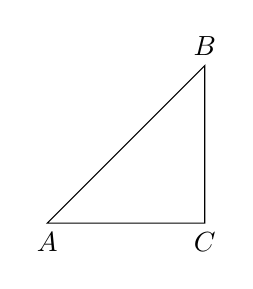
\begin{tikzpicture}
                \draw (0,0) node[anchor=north]{$A$}
                -- (2,0) node[anchor=north]{$C$}
                -- (2,2) node[anchor=south]{$B$} -- cycle;
        \end{tikzpicture}
\end{wrapfigure}
%TODO INDICAR EL CALCULO DE ánguloS, TRASLACION DE ánguloS DE UN CUADRANTE A OTRO, PROPIEDADES DE ánguloS AL SUMAR, RESTAR, ETC%
 Veremos como calcular las funciones trigonométricas y posteriormente algunas de sus propiedades
\begin{itemize}
        \item \(\bm{\sin{\bm{\alpha}} = \frac{\overline{BC}}{\overline{AB}}}\)
        \item \(\bm{\cos{\bm{\alpha}} = \frac{\overline{AC}}{\overline{AB}}}\)
        \item \(\bm{\tan{\bm{\alpha}} = \frac{\overline{BC}}{\overline{AC}}}\)
        \item \(\bm{\csc{\bm{\alpha}} = \sin{\bm{\alpha}}^{-1}=\frac{\overline{AB}}{\overline{BC}}}\)
        \item \(\bm{\sec{\bm{\alpha}} = \cos{\bm{\alpha}}^{-1}=\frac{\overline{AB}}{\overline{AC}}}\)
        \item \(\bm{\cot{\bm{\alpha}} = \tan{\bm{\alpha}}^{-1}=\frac{\overline{AC}}{\overline{BC}}}\)
\end{itemize}
Al hablar en trigonometría usaremos los radianes \(\bm{k\pi}\) \textbf{rad} y en función del ángulo que tengamos, lo podemos simplificar a otro que sea inferior a \(\frac{\pi}{2}\) rad:
\begin{itemize}
        \item {\boldmath \(\sin{(\frac{\pi}{2} \pm \alpha)} = \cos{\alpha}\)}
        \item {\boldmath \(\cos{(\frac{\pi}{2} \pm \alpha)} = \mp\sin{\alpha}\)}
        \item {\boldmath \(\sin{(\pi \pm \alpha)} = \mp\sin{\alpha}\)}
        \item {\boldmath \(\cos{(\pi \pm \alpha)} = -\cos{\alpha}\)}
        \item {\boldmath \(\sin{(3\frac{\pi}{2} \pm \alpha)} = -\cos{\alpha}\)}
        \item {\boldmath \(\cos{(3\frac{\pi}{2} \pm \alpha)} = \mp\sin{\alpha}\)}
\end{itemize}
\subsection{Números Complejos}
 Denominamos un número complejo aquel formado por una parte real \(\mathbf{\Re(z)}\) y una imaginaria \(\mathbf{\Im(z)}\).
\[
        \boxed{ z = a\pm bj \hspace{5mm} \textnormal{Siendo j = \(\sqrt{-1}\), a veces se representa con \(i\)}}
\]
Podemos denominar el complementario de un número complejo como aquel cuya parte imaginaria tiene el signo opuesto, se suele representar como, \(\mathbf{\overline{z}}\)
\subsubsection{Operaciones}
\begin{itemize}
        \item Sumas y restas: Se suma la parte real y la imaginaria por separado.
        \item Multiplicación: Será más sencillo expresarlos como fasores, sumando los ángulos y multiplicando las amplitudes.
        \item División: Al igual que con la multiplicación, es más sencillo expresarlo como fasores, se restan los ángulos (numerador menos denominador) y se dividen las amplitudes,
\end{itemize}
\subsection{Fasores}
 Dado un número complejo \(\mathbf{z = a + bj}\), su expresión como fasor se basa usando el \underline{número de Euler}, a la que podemos llegar utilizando la:
\[
        \boxed{z = \left | z \right |e^{\rho j}}
\]
 Siendo \(\mathbf{\rho}\) el ángulo que entre el coeficiente de la parte imaginaria y el de la parte real, denominado \underline{argumento} y \(\mathbf{\left | z \right |}\) es el\underline{módulo} entre la parte real y la imaginaria.
\[\boxed{
                \rho = \arctan{(\frac{b}{a})} \hspace{5mm} \textnormal{Siempre se expresará en radianes}}
\]
\[
        \boxed{\left | z \right |=\sqrt{a^2 - (bj)^2} = \sqrt{a^2+ b^2}}
\]
 Finalmente podemos decir que esta expresión se denomina forma polar, y podemos traspasarla a una forma usando razones trigonométricas, por lo que:
\[
        \boxed{z = a + bj \hspace{3mm} \Rightarrow \hspace{3mm}\tilde{z} = \left | z \right |e^{\rho j} \hspace{1.5mm}=\hspace{1.5mm}\left | z \right | \cos{(wt + \rho)}}
\]